\documentclass[10pt]{article}
\usepackage{tmlr}
% For arXiv: \usepackage[preprint]{tmlr}
%%%%% NEW MATH DEFINITIONS %%%%%

\usepackage{amsmath,amsfonts,bm}

% Mark sections of captions for referring to divisions of figures
\newcommand{\figleft}{{\em (Left)}}
\newcommand{\figcenter}{{\em (Center)}}
\newcommand{\figright}{{\em (Right)}}
\newcommand{\figtop}{{\em (Top)}}
\newcommand{\figbottom}{{\em (Bottom)}}
\newcommand{\captiona}{{\em (a)}}
\newcommand{\captionb}{{\em (b)}}
\newcommand{\captionc}{{\em (c)}}
\newcommand{\captiond}{{\em (d)}}

% Highlight a newly defined term
\newcommand{\newterm}[1]{{\bf #1}}


% Figure reference, lower-case.
\def\figref#1{figure~\ref{#1}}
% Figure reference, capital. For start of sentence
\def\Figref#1{Figure~\ref{#1}}
\def\twofigref#1#2{figures \ref{#1} and \ref{#2}}
\def\quadfigref#1#2#3#4{figures \ref{#1}, \ref{#2}, \ref{#3} and \ref{#4}}
% Section reference, lower-case.
\def\secref#1{section~\ref{#1}}
% Section reference, capital.
\def\Secref#1{Section~\ref{#1}}
% Reference to two sections.
\def\twosecrefs#1#2{sections \ref{#1} and \ref{#2}}
% Reference to three sections.
\def\secrefs#1#2#3{sections \ref{#1}, \ref{#2} and \ref{#3}}
% Reference to an equation, lower-case.
\def\eqref#1{equation~\ref{#1}}
% Reference to an equation, upper case
\def\Eqref#1{Equation~\ref{#1}}
% A raw reference to an equation---avoid using if possible
\def\plaineqref#1{\ref{#1}}
% Reference to a chapter, lower-case.
\def\chapref#1{chapter~\ref{#1}}
% Reference to an equation, upper case.
\def\Chapref#1{Chapter~\ref{#1}}
% Reference to a range of chapters
\def\rangechapref#1#2{chapters\ref{#1}--\ref{#2}}
% Reference to an algorithm, lower-case.
\def\algref#1{algorithm~\ref{#1}}
% Reference to an algorithm, upper case.
\def\Algref#1{Algorithm~\ref{#1}}
\def\twoalgref#1#2{algorithms \ref{#1} and \ref{#2}}
\def\Twoalgref#1#2{Algorithms \ref{#1} and \ref{#2}}
% Reference to a part, lower case
\def\partref#1{part~\ref{#1}}
% Reference to a part, upper case
\def\Partref#1{Part~\ref{#1}}
\def\twopartref#1#2{parts \ref{#1} and \ref{#2}}

\def\ceil#1{\lceil #1 \rceil}
\def\floor#1{\lfloor #1 \rfloor}
\def\1{\bm{1}}
\newcommand{\train}{\mathcal{D}}
\newcommand{\valid}{\mathcal{D_{\mathrm{valid}}}}
\newcommand{\test}{\mathcal{D_{\mathrm{test}}}}

\def\eps{{\epsilon}}


% Random variables
\def\reta{{\textnormal{$\eta$}}}
\def\ra{{\textnormal{a}}}
\def\rb{{\textnormal{b}}}
\def\rc{{\textnormal{c}}}
\def\rd{{\textnormal{d}}}
\def\re{{\textnormal{e}}}
\def\rf{{\textnormal{f}}}
\def\rg{{\textnormal{g}}}
\def\rh{{\textnormal{h}}}
\def\ri{{\textnormal{i}}}
\def\rj{{\textnormal{j}}}
\def\rk{{\textnormal{k}}}
\def\rl{{\textnormal{l}}}
% rm is already a command, just don't name any random variables m
\def\rn{{\textnormal{n}}}
\def\ro{{\textnormal{o}}}
\def\rp{{\textnormal{p}}}
\def\rq{{\textnormal{q}}}
\def\rr{{\textnormal{r}}}
\def\rs{{\textnormal{s}}}
\def\rt{{\textnormal{t}}}
\def\ru{{\textnormal{u}}}
\def\rv{{\textnormal{v}}}
\def\rw{{\textnormal{w}}}
\def\rx{{\textnormal{x}}}
\def\ry{{\textnormal{y}}}
\def\rz{{\textnormal{z}}}

% Random vectors
\def\rvepsilon{{\mathbf{\epsilon}}}
\def\rvtheta{{\mathbf{\theta}}}
\def\rva{{\mathbf{a}}}
\def\rvb{{\mathbf{b}}}
\def\rvc{{\mathbf{c}}}
\def\rvd{{\mathbf{d}}}
\def\rve{{\mathbf{e}}}
\def\rvf{{\mathbf{f}}}
\def\rvg{{\mathbf{g}}}
\def\rvh{{\mathbf{h}}}
\def\rvu{{\mathbf{i}}}
\def\rvj{{\mathbf{j}}}
\def\rvk{{\mathbf{k}}}
\def\rvl{{\mathbf{l}}}
\def\rvm{{\mathbf{m}}}
\def\rvn{{\mathbf{n}}}
\def\rvo{{\mathbf{o}}}
\def\rvp{{\mathbf{p}}}
\def\rvq{{\mathbf{q}}}
\def\rvr{{\mathbf{r}}}
\def\rvs{{\mathbf{s}}}
\def\rvt{{\mathbf{t}}}
\def\rvu{{\mathbf{u}}}
\def\rvv{{\mathbf{v}}}
\def\rvw{{\mathbf{w}}}
\def\rvx{{\mathbf{x}}}
\def\rvy{{\mathbf{y}}}
\def\rvz{{\mathbf{z}}}

% Elements of random vectors
\def\erva{{\textnormal{a}}}
\def\ervb{{\textnormal{b}}}
\def\ervc{{\textnormal{c}}}
\def\ervd{{\textnormal{d}}}
\def\erve{{\textnormal{e}}}
\def\ervf{{\textnormal{f}}}
\def\ervg{{\textnormal{g}}}
\def\ervh{{\textnormal{h}}}
\def\ervi{{\textnormal{i}}}
\def\ervj{{\textnormal{j}}}
\def\ervk{{\textnormal{k}}}
\def\ervl{{\textnormal{l}}}
\def\ervm{{\textnormal{m}}}
\def\ervn{{\textnormal{n}}}
\def\ervo{{\textnormal{o}}}
\def\ervp{{\textnormal{p}}}
\def\ervq{{\textnormal{q}}}
\def\ervr{{\textnormal{r}}}
\def\ervs{{\textnormal{s}}}
\def\ervt{{\textnormal{t}}}
\def\ervu{{\textnormal{u}}}
\def\ervv{{\textnormal{v}}}
\def\ervw{{\textnormal{w}}}
\def\ervx{{\textnormal{x}}}
\def\ervy{{\textnormal{y}}}
\def\ervz{{\textnormal{z}}}

% Random matrices
\def\rmA{{\mathbf{A}}}
\def\rmB{{\mathbf{B}}}
\def\rmC{{\mathbf{C}}}
\def\rmD{{\mathbf{D}}}
\def\rmE{{\mathbf{E}}}
\def\rmF{{\mathbf{F}}}
\def\rmG{{\mathbf{G}}}
\def\rmH{{\mathbf{H}}}
\def\rmI{{\mathbf{I}}}
\def\rmJ{{\mathbf{J}}}
\def\rmK{{\mathbf{K}}}
\def\rmL{{\mathbf{L}}}
\def\rmM{{\mathbf{M}}}
\def\rmN{{\mathbf{N}}}
\def\rmO{{\mathbf{O}}}
\def\rmP{{\mathbf{P}}}
\def\rmQ{{\mathbf{Q}}}
\def\rmR{{\mathbf{R}}}
\def\rmS{{\mathbf{S}}}
\def\rmT{{\mathbf{T}}}
\def\rmU{{\mathbf{U}}}
\def\rmV{{\mathbf{V}}}
\def\rmW{{\mathbf{W}}}
\def\rmX{{\mathbf{X}}}
\def\rmY{{\mathbf{Y}}}
\def\rmZ{{\mathbf{Z}}}

% Elements of random matrices
\def\ermA{{\textnormal{A}}}
\def\ermB{{\textnormal{B}}}
\def\ermC{{\textnormal{C}}}
\def\ermD{{\textnormal{D}}}
\def\ermE{{\textnormal{E}}}
\def\ermF{{\textnormal{F}}}
\def\ermG{{\textnormal{G}}}
\def\ermH{{\textnormal{H}}}
\def\ermI{{\textnormal{I}}}
\def\ermJ{{\textnormal{J}}}
\def\ermK{{\textnormal{K}}}
\def\ermL{{\textnormal{L}}}
\def\ermM{{\textnormal{M}}}
\def\ermN{{\textnormal{N}}}
\def\ermO{{\textnormal{O}}}
\def\ermP{{\textnormal{P}}}
\def\ermQ{{\textnormal{Q}}}
\def\ermR{{\textnormal{R}}}
\def\ermS{{\textnormal{S}}}
\def\ermT{{\textnormal{T}}}
\def\ermU{{\textnormal{U}}}
\def\ermV{{\textnormal{V}}}
\def\ermW{{\textnormal{W}}}
\def\ermX{{\textnormal{X}}}
\def\ermY{{\textnormal{Y}}}
\def\ermZ{{\textnormal{Z}}}

% Vectors
\def\vzero{{\bm{0}}}
\def\vone{{\bm{1}}}
\def\vmu{{\bm{\mu}}}
\def\vtheta{{\bm{\theta}}}
\def\va{{\bm{a}}}
\def\vb{{\bm{b}}}
\def\vc{{\bm{c}}}
\def\vd{{\bm{d}}}
\def\ve{{\bm{e}}}
\def\vf{{\bm{f}}}
\def\vg{{\bm{g}}}
\def\vh{{\bm{h}}}
\def\vi{{\bm{i}}}
\def\vj{{\bm{j}}}
\def\vk{{\bm{k}}}
\def\vl{{\bm{l}}}
\def\vm{{\bm{m}}}
\def\vn{{\bm{n}}}
\def\vo{{\bm{o}}}
\def\vp{{\bm{p}}}
\def\vq{{\bm{q}}}
\def\vr{{\bm{r}}}
\def\vs{{\bm{s}}}
\def\vt{{\bm{t}}}
\def\vu{{\bm{u}}}
\def\vv{{\bm{v}}}
\def\vw{{\bm{w}}}
\def\vx{{\bm{x}}}
\def\vy{{\bm{y}}}
\def\vz{{\bm{z}}}

% Elements of vectors
\def\evalpha{{\alpha}}
\def\evbeta{{\beta}}
\def\evepsilon{{\epsilon}}
\def\evlambda{{\lambda}}
\def\evomega{{\omega}}
\def\evmu{{\mu}}
\def\evpsi{{\psi}}
\def\evsigma{{\sigma}}
\def\evtheta{{\theta}}
\def\eva{{a}}
\def\evb{{b}}
\def\evc{{c}}
\def\evd{{d}}
\def\eve{{e}}
\def\evf{{f}}
\def\evg{{g}}
\def\evh{{h}}
\def\evi{{i}}
\def\evj{{j}}
\def\evk{{k}}
\def\evl{{l}}
\def\evm{{m}}
\def\evn{{n}}
\def\evo{{o}}
\def\evp{{p}}
\def\evq{{q}}
\def\evr{{r}}
\def\evs{{s}}
\def\evt{{t}}
\def\evu{{u}}
\def\evv{{v}}
\def\evw{{w}}
\def\evx{{x}}
\def\evy{{y}}
\def\evz{{z}}

% Matrix
\def\mA{{\bm{A}}}
\def\mB{{\bm{B}}}
\def\mC{{\bm{C}}}
\def\mD{{\bm{D}}}
\def\mE{{\bm{E}}}
\def\mF{{\bm{F}}}
\def\mG{{\bm{G}}}
\def\mH{{\bm{H}}}
\def\mI{{\bm{I}}}
\def\mJ{{\bm{J}}}
\def\mK{{\bm{K}}}
\def\mL{{\bm{L}}}
\def\mM{{\bm{M}}}
\def\mN{{\bm{N}}}
\def\mO{{\bm{O}}}
\def\mP{{\bm{P}}}
\def\mQ{{\bm{Q}}}
\def\mR{{\bm{R}}}
\def\mS{{\bm{S}}}
\def\mT{{\bm{T}}}
\def\mU{{\bm{U}}}
\def\mV{{\bm{V}}}
\def\mW{{\bm{W}}}
\def\mX{{\bm{X}}}
\def\mY{{\bm{Y}}}
\def\mZ{{\bm{Z}}}
\def\mBeta{{\bm{\beta}}}
\def\mPhi{{\bm{\Phi}}}
\def\mLambda{{\bm{\Lambda}}}
\def\mSigma{{\bm{\Sigma}}}

% Tensor
\DeclareMathAlphabet{\mathsfit}{\encodingdefault}{\sfdefault}{m}{sl}
\SetMathAlphabet{\mathsfit}{bold}{\encodingdefault}{\sfdefault}{bx}{n}
\newcommand{\tens}[1]{\bm{\mathsfit{#1}}}
\def\tA{{\tens{A}}}
\def\tB{{\tens{B}}}
\def\tC{{\tens{C}}}
\def\tD{{\tens{D}}}
\def\tE{{\tens{E}}}
\def\tF{{\tens{F}}}
\def\tG{{\tens{G}}}
\def\tH{{\tens{H}}}
\def\tI{{\tens{I}}}
\def\tJ{{\tens{J}}}
\def\tK{{\tens{K}}}
\def\tL{{\tens{L}}}
\def\tM{{\tens{M}}}
\def\tN{{\tens{N}}}
\def\tO{{\tens{O}}}
\def\tP{{\tens{P}}}
\def\tQ{{\tens{Q}}}
\def\tR{{\tens{R}}}
\def\tS{{\tens{S}}}
\def\tT{{\tens{T}}}
\def\tU{{\tens{U}}}
\def\tV{{\tens{V}}}
\def\tW{{\tens{W}}}
\def\tX{{\tens{X}}}
\def\tY{{\tens{Y}}}
\def\tZ{{\tens{Z}}}


% Graph
\def\gA{{\mathcal{A}}}
\def\gB{{\mathcal{B}}}
\def\gC{{\mathcal{C}}}
\def\gD{{\mathcal{D}}}
\def\gE{{\mathcal{E}}}
\def\gF{{\mathcal{F}}}
\def\gG{{\mathcal{G}}}
\def\gH{{\mathcal{H}}}
\def\gI{{\mathcal{I}}}
\def\gJ{{\mathcal{J}}}
\def\gK{{\mathcal{K}}}
\def\gL{{\mathcal{L}}}
\def\gM{{\mathcal{M}}}
\def\gN{{\mathcal{N}}}
\def\gO{{\mathcal{O}}}
\def\gP{{\mathcal{P}}}
\def\gQ{{\mathcal{Q}}}
\def\gR{{\mathcal{R}}}
\def\gS{{\mathcal{S}}}
\def\gT{{\mathcal{T}}}
\def\gU{{\mathcal{U}}}
\def\gV{{\mathcal{V}}}
\def\gW{{\mathcal{W}}}
\def\gX{{\mathcal{X}}}
\def\gY{{\mathcal{Y}}}
\def\gZ{{\mathcal{Z}}}

% Sets
\def\sA{{\mathbb{A}}}
\def\sB{{\mathbb{B}}}
\def\sC{{\mathbb{C}}}
\def\sD{{\mathbb{D}}}
% Don't use a set called E, because this would be the same as our symbol
% for expectation.
\def\sF{{\mathbb{F}}}
\def\sG{{\mathbb{G}}}
\def\sH{{\mathbb{H}}}
\def\sI{{\mathbb{I}}}
\def\sJ{{\mathbb{J}}}
\def\sK{{\mathbb{K}}}
\def\sL{{\mathbb{L}}}
\def\sM{{\mathbb{M}}}
\def\sN{{\mathbb{N}}}
\def\sO{{\mathbb{O}}}
\def\sP{{\mathbb{P}}}
\def\sQ{{\mathbb{Q}}}
\def\sR{{\mathbb{R}}}
\def\sS{{\mathbb{S}}}
\def\sT{{\mathbb{T}}}
\def\sU{{\mathbb{U}}}
\def\sV{{\mathbb{V}}}
\def\sW{{\mathbb{W}}}
\def\sX{{\mathbb{X}}}
\def\sY{{\mathbb{Y}}}
\def\sZ{{\mathbb{Z}}}

% Entries of a matrix
\def\emLambda{{\Lambda}}
\def\emA{{A}}
\def\emB{{B}}
\def\emC{{C}}
\def\emD{{D}}
\def\emE{{E}}
\def\emF{{F}}
\def\emG{{G}}
\def\emH{{H}}
\def\emI{{I}}
\def\emJ{{J}}
\def\emK{{K}}
\def\emL{{L}}
\def\emM{{M}}
\def\emN{{N}}
\def\emO{{O}}
\def\emP{{P}}
\def\emQ{{Q}}
\def\emR{{R}}
\def\emS{{S}}
\def\emT{{T}}
\def\emU{{U}}
\def\emV{{V}}
\def\emW{{W}}
\def\emX{{X}}
\def\emY{{Y}}
\def\emZ{{Z}}
\def\emSigma{{\Sigma}}

% entries of a tensor
% Same font as tensor, without \bm wrapper
\newcommand{\etens}[1]{\mathsfit{#1}}
\def\etLambda{{\etens{\Lambda}}}
\def\etA{{\etens{A}}}
\def\etB{{\etens{B}}}
\def\etC{{\etens{C}}}
\def\etD{{\etens{D}}}
\def\etE{{\etens{E}}}
\def\etF{{\etens{F}}}
\def\etG{{\etens{G}}}
\def\etH{{\etens{H}}}
\def\etI{{\etens{I}}}
\def\etJ{{\etens{J}}}
\def\etK{{\etens{K}}}
\def\etL{{\etens{L}}}
\def\etM{{\etens{M}}}
\def\etN{{\etens{N}}}
\def\etO{{\etens{O}}}
\def\etP{{\etens{P}}}
\def\etQ{{\etens{Q}}}
\def\etR{{\etens{R}}}
\def\etS{{\etens{S}}}
\def\etT{{\etens{T}}}
\def\etU{{\etens{U}}}
\def\etV{{\etens{V}}}
\def\etW{{\etens{W}}}
\def\etX{{\etens{X}}}
\def\etY{{\etens{Y}}}
\def\etZ{{\etens{Z}}}

% The true underlying data generating distribution
\newcommand{\pdata}{p_{\rm{data}}}
% The empirical distribution defined by the training set
\newcommand{\ptrain}{\hat{p}_{\rm{data}}}
\newcommand{\Ptrain}{\hat{P}_{\rm{data}}}
% The model distribution
\newcommand{\pmodel}{p_{\rm{model}}}
\newcommand{\Pmodel}{P_{\rm{model}}}
\newcommand{\ptildemodel}{\tilde{p}_{\rm{model}}}
% Stochastic autoencoder distributions
\newcommand{\pencode}{p_{\rm{encoder}}}
\newcommand{\pdecode}{p_{\rm{decoder}}}
\newcommand{\precons}{p_{\rm{reconstruct}}}

\newcommand{\laplace}{\mathrm{Laplace}} % Laplace distribution

\newcommand{\E}{\mathbb{E}}
\newcommand{\Ls}{\mathcal{L}}
\newcommand{\R}{\mathbb{R}}
\newcommand{\emp}{\tilde{p}}
\newcommand{\lr}{\alpha}
\newcommand{\reg}{\lambda}
\newcommand{\rect}{\mathrm{rectifier}}
\newcommand{\softmax}{\mathrm{softmax}}
\newcommand{\sigmoid}{\sigma}
\newcommand{\softplus}{\zeta}
\newcommand{\KL}{D_{\mathrm{KL}}}
\newcommand{\Var}{\mathrm{Var}}
\newcommand{\standarderror}{\mathrm{SE}}
\newcommand{\Cov}{\mathrm{Cov}}
% Wolfram Mathworld says $L^2$ is for function spaces and $\ell^2$ is for vectors
% But then they seem to use $L^2$ for vectors throughout the site, and so does
% wikipedia.
\newcommand{\normlzero}{L^0}
\newcommand{\normlone}{L^1}
\newcommand{\normltwo}{L^2}
\newcommand{\normlp}{L^p}
\newcommand{\normmax}{L^\infty}

\newcommand{\parents}{Pa} % See usage in notation.tex. Chosen to match Daphne's book.

\DeclareMathOperator*{\argmax}{arg\,max}
\DeclareMathOperator*{\argmin}{arg\,min}

\DeclareMathOperator{\sign}{sign}
\DeclareMathOperator{\Tr}{Tr}
\let\ab\allowbreak

\usepackage{hyperref}
\usepackage{url}
\usepackage{booktabs}
\usepackage{xcolor}
\usepackage{graphicx}
\usepackage{amsmath}

% cleveref is not installed here: \cref / \Cref map to hyperref's \autoref with capitalized names
\newcommand{\cref}[1]{\autoref{#1}}
\newcommand{\Cref}[1]{\autoref{#1}}
\renewcommand{\sectionautorefname}{Section}
\renewcommand{\subsectionautorefname}{Section}
\renewcommand{\tableautorefname}{Table}
\renewcommand{\figureautorefname}{Figure}
\newcommand{\tf}{Tree Forcing}
% Visible placeholder for results that are still running or text the authors will write.
\newcommand{\pending}[1]{\textcolor{red}{[#1]}}

\title{Tree Forcing: Training Single-Pass Decision Models\\on the Intermediate Conclusions of Verified Reasoning Trees}

% Authors are hidden by tmlr.sty in the submission build; they appear with [preprint] (arXiv) or [accepted].
\author{\name Haotian Yang\thanks{Equal contribution.} \email haotian.yang@studbocconi.it \\
      \addr Bocconi University
      \AND
      \name Haoyu Zhang\footnotemark[1] \email hzhang2359@wisc.edu \\
      \addr University of Wisconsin--Madison}

\def\month{MM}
\def\year{YYYY}
\def\openreview{\url{https://openreview.net/forum?id=XXXX}}

\begin{document}
\maketitle

\begin{abstract}
Single-pass decision models read their answer from the probability of each option after one forward pass. This makes
them cheap, but it leaves no room for the intermediate steps that chain-of-thought reasoning writes down. We introduce
\tf{}, a training recipe that turns each intermediate conclusion of a verified reasoning tree into an extra yes/no
question about the problem, answered with the same single-pass readout as the final decision; at test time the model
sees only the final question. On Knights-and-Knaves logic puzzles, \tf{} raises the one-pass accuracy of a 4B model
by 3.7 points over answer-only training with twice the epochs, at all six seeds, and the gain holds at a lower
learning rate, under a KL penalty and at 9B, although its size varies between runs. The gain needs dense, correct
conclusions from the derivation: it disappears when the node answers are permuted, when only three nodes per puzzle
are kept, and when the nodes are replaced by as many correct questions that do not come from the tree. Training the
model to write out the same proof does not help. The trained models also transfer better to BIG-Bench Hard and stay
better calibrated there. On grade-school math, whose trees are sparse and whose steps form serial chains, the gain
is about one point. A single pass, we find, can use intermediate values written into its prompt but computes few of
them on its own, which is consistent with a limit on serial computation; node density, however, remains a confound
that our experiments cannot remove.
\end{abstract}

% =====================================================================================================================
\section{Introduction}
\label{sec:intro}

Large language models are increasingly used as components that make decisions rather than write text: they route
requests, flag policy violations, choose tools and judge the outputs of other models. Recent work proposes to serve
such decisions with a \emph{single-pass} readout, in which the model reads the problem once and the probability it
assigns to each option is taken as its decision \citep{ldm2026}. Single-pass decision models are fast, and they return
a distribution over the options that can be inspected and calibrated.

The price of a single pass is reasoning. Chain-of-thought prompting improves accuracy on multi-step problems by letting
the model write intermediate results before it answers \citep{wei2022cot}, and theoretical work explains why a
transformer of fixed depth can compute more when it may condition on its own intermediate tokens
\citep{feng2023mystery,merrill2024expressive}. A model that answers in one pass has no such scratchpad, and a recent
study of a deployed single-pass decision model shows the consequence: it answers a familiar probability problem
correctly but violates the same rule on an adapted version, and its answers shift with irrelevant numbers and with the
order of the options \citep{imperatrice2026jevbias}. We therefore ask how much of the value of reasoning data can be
moved into training while the deployed model still answers in one pass.

Existing answers mostly supervise the final output or the rationale as text. Answer-only fine-tuning trains on the gold
decision, distillation trains on the answers of a reasoning teacher \citep{yu2024system2}, and methods that use the
rationale itself train the model to generate it, as an auxiliary task \citep{hsieh2023dss,li2022explanations} or as
the output \citep{ho2023teachers,shridhar2023socratic}. Closest to our work, DAIS trains on intermediate
question-answer records extracted from teacher rationales, each conditioned on the answers to earlier sub-questions
\citep{dais2026}. We argue that a single-pass model needs a different kind of supervision: it should be asked for the
intermediate conclusions on which its answer depends, in the format in which its answer is read out, and it should
have to compute these conclusions from the problem rather than read them from its prompt.

In this work, we introduce \tf{}. Given a training problem and a verified reasoning tree, i.e., a set of intermediate
conclusions with known truth values and the dependencies between them, \tf{} turns every node into an extra yes/no
question (``If Alice were a knight, would Henry's statement be false?''), asks it in the context of the problem, and
trains the model to answer it with the same readout as the final decision. No intermediate result is ever written into
a prompt. At test time nothing changes: the model answers the final question alone, so the reasoning annotation is
spent at training time and the single-pass interface stays untouched.

We evaluate \tf{} with Qwen3.5-4B on Knights-and-Knaves puzzles \citep{xie2024kk}, whose trees come from a solver,
and on GSM8K word problems \citep{cobbe2021gsm8k}, whose trees come from the dataset's step annotations, and we compare
against answer-only training on the same problems, paired by seed. Several analyses had their criteria fixed before their
results existed, and we report them whether or not they met them. We find that:
\begin{itemize}
  \item \textbf{On logic puzzles, \tf{} helps.} It raises one-pass accuracy on Knights-and-Knaves at all six seeds,
  across learning rates and a KL penalty, and with a 9B model (\cref{sec:kk}).
  \item \textbf{The gain needs dense, correct conclusions from the derivation.} Permuting the node answers, keeping
  only three nodes per puzzle, or replacing the nodes by other correct questions removes it, and training the model to
  write out the same proof does not help (\cref{sec:content}).
  \item \textbf{The models transfer and stay calibrated.} \tf{} models are more accurate on BIG-Bench Hard and much
  better calibrated on the tasks they were not trained on (\cref{sec:transfer}).
  \item \textbf{It helps little on serial arithmetic.} On GSM8K and on logic grid puzzles the gain is small. A
  single pass can use written intermediate values but computes few of them itself, which may explain this, although
  sparse trees offer a second explanation (Sections~\ref{sec:gsm8k} and~\ref{sec:mechanism}).
\end{itemize}

% =====================================================================================================================
\section{Tree Forcing}
\label{sec:method}

\paragraph{Single-pass decisions.} We consider problems with a fixed set of options. The model reads the problem, the
options labelled A, B, \ldots{} and the string ``Answer:'', and its decision is the distribution over the option
letters at the next position. Answer-only training minimizes the cross-entropy between this distribution and the gold
option, with label smoothing of 0.1.

\paragraph{Reasoning trees.} For every training problem we assume a reasoning tree: a set of intermediate conclusions
whose truth is known, together with the conclusions each one depends on. On Knights-and-Knaves the tree is the trace of
a solver that reads each statement, makes the case splits a person would make and derives what follows in each case
(\cref{fig:example}). On GSM8K a node is a solution step, phrased as the sub-question of the dataset's Socratic
annotation and checked against its calculator note. The trees are used only for training; none is built or consulted
at test time.

\paragraph{Node questions.} We turn each node into a yes/no question. On Knights-and-Knaves a node is a proposition,
and its question asks whether it holds; on GSM8K the question states a candidate value for a step (``How many nickels
did Quentavious spend? Is it 3?''), and every true candidate is paired with a false one. We ask each node question
after the problem statement, with the final question and its options removed, and without the results of the node's
parents, so the model cannot copy an intermediate result from its prompt. Each node question is a separate training
example in the same single-pass format as the final decision.

\paragraph{Training and inference.} Each optimizer update covers a fixed number of problems and includes, for \tf{},
the final question of each problem together with all of its node questions; the node questions of a problem share the
same total loss weight as its final question. The tree generates the node questions, verifies their answers and removes
questions that would reveal the final answer, but its edges do not enter the loss, so the name refers to the source of
the supervision rather than to a structured objective. At test time the model sees exactly what an answer-only model
sees.

\begin{figure}[t]
\centering
\footnotesize
\fbox{\begin{minipage}{0.95\linewidth}
\textbf{Final question (train and test).} On an island, knights always tell the truth and knaves always lie. Each of
the 4 inhabitants below is either a knight or a knave.\\
-- Alice says: ``If Karen is a knight, then Grace is a knave.'' \quad
-- Karen says: ``Alice is a knave or Grace is a knave.''\\
-- Henry says: ``Karen is a knight and Alice is a knave.'' \quad
-- Grace says: ``If Karen is a knight, then Alice is a knight.''\\
Question: Who is a knight and who is a knave? \quad A) \ldots \quad F) \ldots \quad Answer: \textbf{gold letter}\\[4pt]
\textbf{Node questions (train only), asked after the statements.}\\
\emph{Read:} Is Karen a knight exactly when ``Alice is a knave or Grace is a knave.'' is true? \; A) Yes \; B) No
\; Answer: \textbf{A}\\
\emph{Case:} If Alice were a knight, would the statement by Henry, ``Karen is a knight and Alice is a knave.'', be
false? \; A) Yes \; B) No \; Answer: \textbf{A}\\
\emph{Derive:} \ldots{} (44 node questions per puzzle on average)
\end{minipage}}
\caption{A Knights-and-Knaves training problem and two of its node questions.}
\label{fig:example}
\end{figure}

% =====================================================================================================================
\section{Experimental Setup}
\label{sec:setup}

\paragraph{Tasks.} Our Knights-and-Knaves (K\&K) training set has 1,792 generated puzzles with 4 to 10 inhabitants and
six options each, every option a full assignment of roles; the solver trees have 44 nodes per puzzle on average, of
which about half take a case, a third derive a consequence and the rest read a statement. Our main test set,
\emph{K\&K-Deep}, has 2,000 puzzles with 4 to 20 inhabitants, most of them larger than any training puzzle. We also
report a smaller held-out set (\emph{K\&K-Held-out}) and \emph{K\&K-External}, the public puzzles of
\citet{xie2024kk}, which are worded differently from ours. For GSM8K we turn 5,923 training problems into five-option
decisions, with 2.5 node questions per problem, and test on GSM8K and GSM1K \citep{zhang2024gsm1k} with two kinds of
distractors: \emph{original} ones built from the problem's numbers and \emph{cue-free} ones taken from other problems.

\paragraph{Training.} We fine-tune all parameters of Qwen3.5-4B, the post-trained release, with AdamW at a learning
rate of $3\cdot10^{-6}$ (\cref{app:training}). On K\&K, \tf{} trains for 6 epochs and answer-only training for 12, and
for each method we keep the epoch with the best validation accuracy averaged over its seeds (5 and 9). On GSM8K, the
cue-free validation set chooses between 1 and 2 epochs for each method and picks 1 for both. Twice the epochs is not
twice the compute: with its node questions, a \tf{} run on K\&K costs about 2.9 times the GPU hours of an
answer-only run, once, at training time.

\paragraph{Controls.} Besides answer-only training, we compare against variants that change one thing at a time:
\emph{permuted nodes} keeps every node question but permutes the answers within each problem; \emph{three} and
\emph{eight nodes} keep a fixed subset of each puzzle's nodes at the same total weight; \emph{read nodes only} keeps
the nodes that read a statement; the \emph{verification control} replaces the nodes by as many correct questions that
are not from the tree, each asking whether a statement is true under a random assignment of roles that is neither the
solution nor an option; \emph{proof generation} trains the model to write out the solver's proof as text, in our
training loop as well (\emph{tree batching}); and the \emph{DAIS-style} control states the parents' answers in every
derived node question, as DAIS does \citep{dais2026}.

\paragraph{Statistics.} We report means over seeds and differences paired by seed. We call a difference significant
only when both a seed-level $t$ interval and a two-level bootstrap interval over seeds and test problems exclude zero;
the intervals and per-seed values are in \cref{app:perseed}.

% =====================================================================================================================
\section{Results}
\label{sec:results}

\subsection{Knights-and-Knaves}
\label{sec:kk}

\Cref{tab:kk} shows the main result. On K\&K-Deep, \tf{} answers 73.7\% of the puzzles correctly in one pass, against
69.9\% for answer-only training, and it is ahead at every one of the six seeds. The gain does not depend on the
learning rate or on how far the model drifts from its initialization, and it holds with a 9B model, where \tf{} is
ahead at all three seeds. It is similar within the training range of puzzle sizes and beyond it, and largest on the
externally worded puzzles of K\&K-External, while on the small K\&K-Held-out set it points the same way without being
significant.

\begin{table}[t]
\centering
\small
\caption{K\&K-Deep accuracy (\%). Bold: significant gain.}
\label{tab:kk}
\begin{tabular}{lcccc}
\toprule
Setting & Answer-only & \tf{} & Gain & Seeds ahead \\
\midrule
4B (main) & 69.9 & 73.7 & $\mathbf{+3.7}$ & 6/6 \\
4B, half the learning rate & 66.7 & 69.7 & $\mathbf{+3.0}$ & 6/6 \\
4B, KL penalty & 68.8 & 72.9 & $\mathbf{+4.1}$ & 6/6 \\
9B & 71.5 & 76.0 & $\mathbf{+4.5}$ & 3/3 \\
\bottomrule
\end{tabular}
\end{table}

The size of the gain, however, varies between training runs. When we re-ran three of the seeds with the same
configuration, the differences were much smaller, between $-0.7$ and $+2.1$ points, and in a study that trained separate runs for each
training length, the two configurations validation selected differed by only 1.1 points. Pooled over all paired runs,
the mean gain stays positive and significant, and on K\&K-External it is 5.6 points (\cref{app:tuning} and \cref{app:replication}).
We conclude that \tf{} reliably improves the one-pass accuracy on these puzzles, but that a single comparison can
overstate or understate how much. For reference, the same model trained to write out the solver's proof before
answering, at about a thousand generated tokens per puzzle, reaches 86.4\% on K\&K-Held-out, where answer-only
training reaches 80.9\% and \tf{} 83.0\% in one pass; \tf{} thus closes about two fifths of the distance between a
single pass and written reasoning on these puzzles.

\subsection{What the gain depends on}
\label{sec:content}

A gain from extra yes/no questions could come from what they ask, or from side effects of asking them, such as more
updates per problem or more exposure to the statements. \Cref{fig:content} separates the two. The first requirement is
that the answers are correct: permuting the answers within each problem, which keeps the questions, their number and
their yes rate, removes the gain entirely.

\begin{figure}[t]
\centering
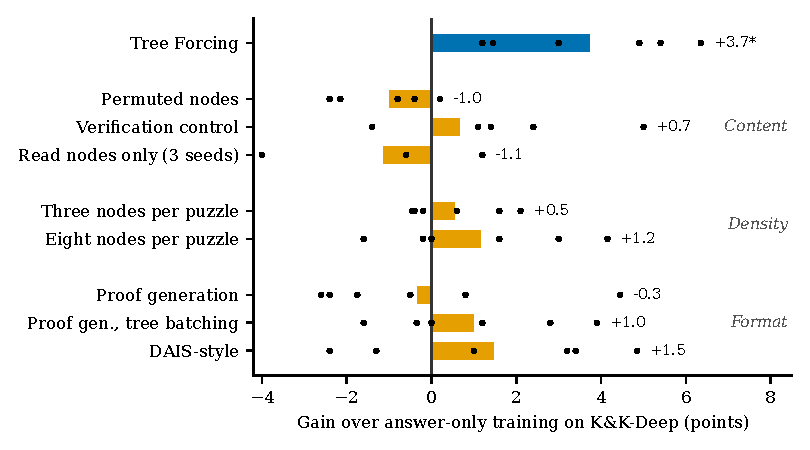
\includegraphics[width=0.78\linewidth]{figures/content.pdf}
\caption{Gain over answer-only training on K\&K-Deep (points; dots: seeds).}
\label{fig:content}
\end{figure}

Correct answers, however, are not enough. The verification control asks as many correct questions about the same
statements, in the same format, but they do not come from the solver's derivation, and it gains less than a point.
Keeping only the nodes that read a statement gives nothing either, so the case and derivation steps carry the effect.
Finally, the supervision has to be dense: with three nodes per puzzle the gain is half a point, with eight about one,
and only the full trees, with 44 nodes on average, give the full gain. We read this as follows: the in-domain gain
comes from training the model on many of the conclusions it has to reach on the way to the answer.

Since the solver's proof states these conclusions too, one may ask whether they need to be posed as questions at all.
In the schemes we tested, they do better that way. Training the model to write out the proof, with the final question
alongside, does not improve its one-pass accuracy; trained inside our own training loop, the proof objective comes
closer, but \tf{} stays ahead. We attribute this to
readout alignment, although the two objectives also differ in target length and density: a proof teaches the model to
produce the next sentence of an argument, which it never does at test time, whereas a node question asks it to hold a
conclusion in the readout it is judged on. Stating the parents' answers in each node question, as DAIS does, brought
no reliable benefit in our setting.

\subsection{Transfer and calibration}
\label{sec:transfer}

Since the trained models are meant to serve as general decision components, we also evaluate the K\&K models, without
further training, on BIG-Bench Hard \citep{suzgun2022bbh}, BIG-Bench Extra Hard \citep{kazemi2025bbeh}, FOLIO
\citep{han2022folio}, MuSR \citep{sprague2023musr}, ShARC \citep{saeidi2018sharc} and GSM8K posed as a
multiple-choice question (\cref{tab:transfer}). On BIG-Bench Hard, answer-only training on K\&K lifts the untrained
model by 2 points and \tf{} by 7, at every seed. On BIG-Bench Extra Hard, ShARC and GSM8K, answer-only training falls
below the untrained model while \tf{} stays near it, so there the difference reflects forgetting rather than transfer.
\tf{} is ahead on five of the six sets, significantly on four. The gain on BIG-Bench Hard holds when both methods train
for the same number of epochs and on tasks with three or more options as well as on two-option tasks, and it is
largest on Web of Lies, the task closest to Knights-and-Knaves (\cref{app:heldout}).

\begin{table}[t]
\centering
\small
\caption{Accuracy (\%) of the K\&K-trained models on tasks they were not trained on.}
\label{tab:transfer}
\begin{tabular}{lccc}
\toprule
Test set & Untrained & Answer-only & \tf{} \\
\midrule
BIG-Bench Hard & 53.1 & 55.4 & \textbf{60.3} \\
BIG-Bench Extra Hard & 23.0 & 20.9 & \textbf{23.4} \\
FOLIO & 55.7 & 53.2 & \textbf{57.1} \\
MuSR & 52.1 & \textbf{58.9} & 58.3 \\
ShARC & \textbf{66.9} & 43.3 & 63.3 \\
GSM8K (multiple choice) & \textbf{42.9} & 38.7 & 41.5 \\
\bottomrule
\end{tabular}
\end{table}

The transfer has weaker requirements than the in-domain gain. It needs correct answers, since the permuted control is
no better than answer-only training on BIG-Bench Hard, but neither many nodes nor nodes from the tree: three nodes per
puzzle and the verification control transfer about as well as \tf{} (\cref{app:ablations}).

K\&K training also changes calibration. Answer-only training makes the model strongly overconfident on the tasks it was
not trained on, with an expected calibration error of 33 on BIG-Bench Hard, while \tf{} keeps it at 11. This effect
does not need correct answers, since the permuted control is almost as well calibrated, and we read it as a
regularizing effect of the many yes/no targets. A temperature fitted on each model's own K\&K validation set removes
the in-domain difference but not the one on BIG-Bench Hard (\cref{app:heldout}). On GSM8K, the calibration of the two
methods is the same.

\subsection{Two further logic tasks}
\label{sec:zebra}

\paragraph{FOLIO.} To try \tf{} on premises written by people, we trained on FOLIO \citep{han2022folio}. We gave its
first-order annotations to the Z3 prover \citep{demoura2008z3}, kept the problems whose prover verdict agrees with the
gold label, and used as nodes the ground atoms that the premises entail or refute. \tf{} answers 82.8\% of the 132
filtered test problems correctly against 78.4\% for answer-only training. The test set is small, and by our rule the
result is inconclusive; on all 203 test problems with FOLIO's own labels the difference (+5.1) is significant.

\paragraph{Logic grid puzzles.} We also trained on generated logic grid (``Zebra'') puzzles that ask for one cell of the
solution, with trees from a solver that records each deduction with its reasons. Here the gain is small: 45.3\%
against 43.9\% on puzzles of the training sizes, ahead at only three of six seeds, short of the criterion we had
fixed in advance, and no gain on larger grids. Answering one cell usually requires
propagating constraints across the whole grid, a long chain of dependent deductions, which places these puzzles closer
to arithmetic than to Knights-and-Knaves. The Zebra-trained \tf{} models still transfer to K\&K-Deep.

\subsection{Grade-school math}
\label{sec:gsm8k}

GSM8K tells a different story. With the original options, \tf{} is 1.2 points ahead of answer-only training (70.5\%
against 69.3\%), a small but significant gain at all six seeds, and with cue-free options the difference is 0.6
points. The permuted-nodes control, which on K\&K removed the whole gain, comes within about a point of \tf{},
and a placebo that replaces each node question by a question about the surface of the problem comes within one to
two points. The gain on
GSM8K is therefore small, and we cannot separate the contribution of correct node answers from noise. The gap that
remains is large: a model of the same base trained to write out a short rationale before answering reaches about 88\%
on the cue-free sets, against 58\% for either single-pass method.

% =====================================================================================================================
\section{Why Knights-and-Knaves and Not Arithmetic}
\label{sec:mechanism}

The two main tasks differ in several respects at once (\cref{tab:confounds}), so their contrast can suggest an
explanation but not establish one. We discuss two candidates, the kind of computation a node asks for and the density
of the trees, and the evidence for each.

\begin{table}[t]
\centering
\small
\caption{How the two main tasks differ.}
\label{tab:confounds}
\begin{tabular}{lll}
\toprule
 & Knights-and-Knaves & GSM8K \\
\midrule
Nodes per problem & 44 & 2.5 \\
Node content & propositions, cases, derivations & values of solution steps \\
Source of the tree & solver & dataset annotation \\
Options & full role assignments & numbers \\
\bottomrule
\end{tabular}
\end{table}

\paragraph{Local checks and serial chains.} A K\&K node is a local check: whether a statement holds under a case can
be decided from a few lines of the problem once the case is fixed. A GSM8K node asks for the value of a step, which
is the end of a chain of earlier operations that the model has to carry out without writing anything down. Results on
fixed-depth transformers \citep{feng2023mystery,merrill2024expressive} motivate the view that such serial computation is
what a single pass does poorly, although they concern expressivity in general and cannot by themselves explain the
size of a gain in a finite experiment. If the view holds, \tf{} asks the GSM8K model for values it cannot compute.

Two experiments support the serial side directly (\cref{fig:mechanism}). On synthetic arithmetic chains, whose options
can only be told apart by following a chain, the answer-only GSM8K model answers one-step questions almost perfectly
but falls to near chance from three steps on. Training on 27,000 distinct chains makes deeper chains learnable within
that format, but the capacity does not carry over to word problems: on GSM8K problems with two steps left to compute,
these models are less accurate than answer-only training. Conversely, when we write the first true steps of a GSM8K
solution into the prompt, the same models used in \cref{sec:gsm8k} improve sharply: with only the last step left to
compute, accuracy rises from about 60\% to more than 83\% for every method, and it falls back as more steps are left to compute. The steps of another problem or a wrong chain lower accuracy, so
the model reads the values rather than their format, and \tf{} models use the given steps no better than answer-only
models. A single pass, in short, can use intermediate values that are written down, but it computes only one or two
of them on its own (\cref{app:mechanism}).

\begin{figure}[t]
\centering
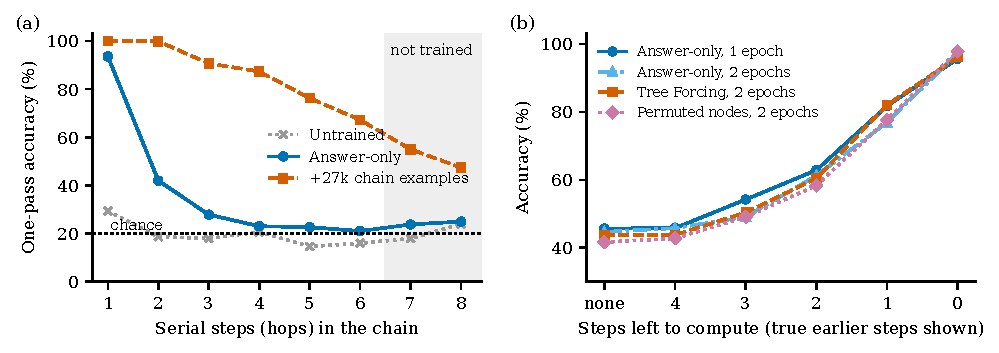
\includegraphics[width=\linewidth]{figures/mechanism.pdf}
\caption{(a) Accuracy on arithmetic chains by number of steps. (b) GSM8K accuracy when the first true steps are shown,
by the number of steps left.}
\label{fig:mechanism}
\end{figure}

The node answers of the trained models agree with this picture. We asked each model the node questions of the
validation problems and compared its node accuracy on the problems it solves with that on the problems it misses. On
K\&K, \tf{} raises node accuracy from 65\% to 84\%, and its node answers are 6 points more accurate on the problems
it solves, against 2 points for answer-only training; the difference persists within each puzzle size. On GSM8K,
\tf{} also raises node accuracy, from 57\% to 64\%, but the relation to the final answer vanishes. This analysis is
observational: it shows that two abilities of the model go together, not that the decision is computed through the
node answers (\cref{app:coupling}).

\paragraph{Density.} The second candidate is simpler. With three nodes per puzzle, close to the 2.5 of GSM8K, the K\&K
gain disappears as well (\cref{sec:content}), so sparse supervision alone could explain why GSM8K gains little. We
cannot make the GSM8K trees denser, since they come from the dataset's annotation, and our experiments therefore do not
decide between the two explanations; both fit the results, and they may act together.

\paragraph{Candidate verification.} Because a K\&K option is a full assignment of roles, a model can in principle check
each candidate against the statements one by one, and most node questions train exactly such checks. We therefore
asked whether \tf{} works by improving the verification of candidates. The gain is not limited to easy candidates: it
is as large on puzzles whose hardest distractor violates a single statement as on the others. Training on verification
itself, however, does not reproduce it, since the verification control asks precisely such questions and gains less
than a point. Whatever \tf{} trains is tied to the conclusions of the derivation rather than to checking statements in
general. A test that offers no full candidates, such as asking for the role of a single inhabitant, would separate
verification from search more cleanly; we leave it to future work.

% =====================================================================================================================
\section{Related Work}
\label{sec:related}

\paragraph{Reasoning without a written chain.} One line of work removes the written chain of thought from generative
models by internalizing it. Implicit chain-of-thought distills the hidden states of a teacher that writes the chain
\citep{deng2023implicit}, stepwise internalization removes the written steps gradually during training
\citep{deng2024internalize}, and Coconut feeds continuous latent states back into the model in place of written steps
\citep{hao2024coconut}. These methods change what the model computes at test time. \tf{} keeps the architecture and
the readout fixed and changes only the training data, for models that read their answer from one position
\citep{ldm2026}.

\paragraph{Rationales as training signal.} A second line trains on the rationale of a teacher or of the model itself:
distilling step by step trains small models to generate rationales as an auxiliary task \citep{hsieh2023dss}, other
work trains on explanations or full reasoning chains \citep{li2022explanations,ho2023teachers,shridhar2023socratic},
and STaR bootstraps rationales from the model's own attempts \citep{zelikman2022star}. In all of these the rationale is
text the model learns to produce; our proof-generation control is the corresponding baseline, and for a model that
answers in one pass it does not help.

\paragraph{Intermediate supervision.} Closest to our work, DAIS \citep{dais2026} extracts sub-questions from teacher
rationales and trains on them as question-answer records, conditioning each on the answers that precede it, and finds
this better than answer-only training and than the same records without the preceding answers. It differs from \tf{}
in three ways: its rationales and sub-questions are generated and checked by a large language model, while our trees
are exact; its models generate their answers, while ours are read out in one pass; and it states the preceding
answers, while \tf{} withholds them. Process supervision \citep{lightman2023verify} also labels intermediate steps, but
to train a reward model for generated solutions, and entailment trees \citep{dalvi2021entailmentbank} provide verified
conclusions for explanation rather than for training a decision.

\paragraph{Knights-and-Knaves.} Knights-and-Knaves puzzles have been used to separate reasoning from memorization in
language models \citep{xie2024kk}. We use them because a solver gives exact trees and because their difficulty grows
with the number of inhabitants.

% =====================================================================================================================
\section{Limitations}
\label{sec:limitations}

Our evidence comes from one model family, at 4B parameters with six seeds and at 9B with three, and the K\&K gain
varies between runs of the same configuration. The gain is clearest on a synthetic task whose trees a solver provides;
on GSM8K, whose trees come from human annotations, it is small, and we have not tested trees that a model would have
to generate. \tf{} needs a tree for every training problem, which limits it to domains where intermediate conclusions
can be stated and verified, and it costs about three times the training compute of answer-only training on K\&K. The
contrast between K\&K and GSM8K is confounded by node density, which we could vary only on K\&K. The node-coupling
analysis is correlational, and the hint experiments show what the models can use, not what they compute internally.

% =====================================================================================================================
\section{Conclusion}
\label{sec:conclusion}

We introduced \tf{}, which trains a single-pass decision model on the intermediate conclusions of verified reasoning
trees, posed as yes/no questions in the format of its final decision. On Knights-and-Knaves, it improves one-pass
accuracy over answer-only training, provided the conclusions are correct, dense and drawn from the derivation, and it
is more effective than training the model to write out the same proof; the trained models also transfer to other
reasoning tasks and stay better calibrated. On grade-school math the gain is small. A single pass can use written
intermediate values but computes few of them itself, which may limit what intermediate supervision can achieve on
serial tasks; whether this, or only the sparsity of the GSM8K trees, explains the small gain is the natural next
question, best answered with tasks that vary dependency depth at a fixed annotation budget.


\bibliography{refs}
\bibliographystyle{tmlr}

\appendix
\renewcommand{\sectionautorefname}{Appendix}

\section{Training Details}
\label{app:training}
\paragraph{Optimization.} We fine-tune all parameters of Qwen3.5-4B (the post-trained release) and Qwen3.5-9B with
AdamW, a learning rate of $3\cdot10^{-6}$ (and $1.5\cdot10^{-6}$ in the learning-rate variant), a cosine schedule after
a linear warm-up over the first 5\% of the updates, and label smoothing of 0.1 on the option-letter targets. The
forward and backward passes run in bf16 under FSDP, with fp32 master weights and the AdamW update on the CPU; the 4B
runs use one GPU (mostly NVIDIA L40S) and the 9B runs two (NVIDIA RTX PRO 6000). The maximum length is 1,536 tokens per
example.
\paragraph{Batches.} On K\&K, an update covers 8 problems; their final and node questions are packed into micro-batches
of at most 4,096 tokens (micro-batch 2, gradient accumulation 4 for the final questions of answer-only training). On
GSM8K, an update covers 32 problems (micro-batch 2, gradient accumulation 16). The node questions of a problem share a
total loss weight of 1, equal to the weight of its final question, and the loss of an update is divided by a constant.
\paragraph{KL variant.} The KL variant adds $0.1\cdot\mathrm{KL}(p\,\|\,p_{\mathrm{ref}})$ over the options of every
training example, where $p_{\mathrm{ref}}$ is the option distribution of the frozen initial model.
\paragraph{Readout and evaluation.} The decision is the distribution over the option letters at the position after
``Answer:''; accuracy counts the most probable letter. We evaluate on validation and the K\&K test sets after every
epoch and on the other test sets at the end of training. Node probes ask the node questions of the validation problems
in their training view and score the yes/no readout.
\paragraph{Proof generation.} The proof of a K\&K puzzle is its solver tree written out as text in topological order
(median 1,166 tokens). The proof-generation model is trained with the final-question loss plus a language-modelling
loss on the proof, conditioned on the problem; it answers in one pass at test time. In the tree-batching variant the
same proof loss is computed in the data loader and normalization of \tf{}, with no node questions.
\paragraph{DAIS-style control.} Every derived node question (not the nodes that read a statement) is asked with the
questions and answers of its parent nodes written as ``Known results:'' under the statements, except where these would
reveal the final answer, throughout training.

\section{Data and Reasoning Trees}
\label{app:data}
\paragraph{Knights-and-Knaves.} Puzzles are generated with 4 to 10 inhabitants (256 per size) and deduplicated against
every evaluation set. A solver reads each statement as a biconditional between the speaker's role and the statement,
takes case splits on roles and derives their consequences; each step becomes a node with its truth value and parents.
Nodes whose question would reveal the final answer are removed. K\&K-Deep (2,000 puzzles) and K\&K-Held-out (450) come from
our puzzle generator, and the training set is deduplicated against both; K\&K-External converts the public test split of \citet{xie2024kk} (2
to 8 inhabitants) into six-option questions whose distractors are wrong assignments that violate the fewest statements,
and drops the 88 puzzles that overlap our training data.
\paragraph{GSM8K.} Trees come from the Socratic annotation: every solution step except the last becomes a node, asked
as its sub-question with the true value and with a wrong value, so that half of the node targets are ``Yes''. Problems
whose calculator notes do not reproduce the gold answer are excluded.
\paragraph{FOLIO.} The first-order annotations of FOLIO are parsed into Z3; a problem is kept when the prover's verdict
(entailed, refuted, undetermined) agrees with the gold label, which holds for 67.6\% of the training problems and
74.6\% of the validation problems among those whose annotations parse into closed formulas. Nodes are ground atoms over the problem's predicates and constants that the premises
entail or refute, rendered as yes/no questions, excluding atoms equivalent to the conclusion. Node questions are
balanced so that, within strata of predicate type and recurring names, ``Yes'' is the answer for half of the questions
of each wording; a logistic regression on the question text alone reaches 46--50\% in story-grouped cross-validation.

\section{Tuning the Baselines}
\label{app:tuning}
\paragraph{Training length on K\&K.} In a tuning study registered before its results, we trained separate runs of
each method at several lengths on seeds 13--15 and selected, for each method, the configuration with the best
seed-mean validation accuracy (\cref{tab:tuning}); the study also included a re-run of the 12-epoch answer-only
schedule. Validation selected 8 epochs for both methods: the 8-epoch \tf{} run and epoch 8 of the re-run 12-epoch
answer-only schedule. The registered comparison of the two selected configurations gave $+1.1$ points on K\&K-Deep (per seed $-2.4$, $+3.1$, $+2.4$;
two-level interval $[-2.2, +3.7]$), $+0.2$ on K\&K-Held-out and $+5.7$ on K\&K-External (two-level interval $[+2.2,
+9.1]$; seed-level interval $[-1.1, +12.4]$). It did not meet its registered criterion on K\&K-Deep.

\begin{table}[h]
\centering
\small
\caption{Training-length study on K\&K (separate runs, seeds 13--15): selected epoch, seed-mean validation accuracy at
that epoch, and K\&K-Deep accuracy at the end of training (\%).}
\label{tab:tuning}
\begin{tabular}{lcccc}
\toprule
Method & Epochs & Selected epoch & Validation & K\&K-Deep (end) \\
\midrule
Answer-only & 2 & 2 & 74.7 & 61.5 \\
 & 4 & 4 & 79.6 & 69.4 \\
 & 8 & 8 & 81.1 & 71.0 \\
 & 12 & 9 & 80.6 & 70.8 \\
 & 12 (re-run) & 8 & 81.6 & 71.8 \\
\tf{} & 3 & 3 & 82.3 & 69.5 \\
 & 4 & 4 & 82.9 & 72.7 \\
 & 6 & 5 & 84.0 & 74.1 \\
 & 8 & 8 & 85.8 & 72.8 \\
\bottomrule
\end{tabular}
\end{table}

\paragraph{Transfer at matched length.} With separate runs of equal length (seeds 13--15, end of training), \tf{} is
ahead on BIG-Bench Hard by 3.1 points at 4 epochs (60.5 versus 57.4) and by 4.2 points at 8 epochs (59.9 versus 55.8),
both significant, and its expected calibration error there is lower (7.0 versus 19.6 and 13.6 versus 31.4).
\paragraph{GSM8K.} On the cue-free validation set, averaged over six seeds, answer-only training reaches 62.8\% after 1
epoch and 62.7\% after 2, and \tf{} 64.8\% after 1 epoch and 64.0\% after 2, so the rule selects 1 epoch for both.
We had first fixed \tf{} at 2 epochs and completed the 1-epoch runs for seeds 16--18 later, with the selection rule
fixed before they ran. At 2 epochs, \tf{} is 1.4 points ahead of 1-epoch answer-only training on the original options
(both intervals above zero) and 0.7 points on the cue-free ones (not significant); at the selected 1 epoch, 1.2
points (significant) and 0.6 points (not significant). Four of the answer-only GSM8K run folders (seeds 15 to 18) were
later overwritten by re-runs of the same configuration; we report the first completed runs, restored from version
history. The written-reasoning reference of \cref{sec:gsm8k} comes from three runs trained to generate the dataset's
rationale (one-pass and generation evaluations of the same runs); on K\&K, from the six proof-generation runs.

\section{All Held-Out Sets}
\label{app:heldout}
\Cref{tab:heldout} lists every held-out set the K\&K-trained models were evaluated on at the end of training, with
the untrained model for reference. Besides the sets of \cref{tab:transfer}, these are two K\&K diagnostic sets. Where \tf{} stays close to the untrained
model while answer-only training falls below it (BIG-Bench Extra Hard, GSM8K, ShARC), we read the difference as
reduced forgetting; where both rise above the untrained model (BIG-Bench Hard), as transfer.

\begin{table}[h]
\centering
\small
\caption{K\&K-trained models (six seeds, end of training) on every held-out set: accuracy (\%) of the untrained model,
answer-only training and \tf{}, and the paired difference; $^\ast$: both 95\% intervals exclude zero.}
\label{tab:heldout}
\begin{tabular}{lrcccc}
\toprule
Test set & Items & Untrained & Answer-only & \tf{} & $\Delta$ \\
\midrule
BIG-Bench Hard & 5,507 & 53.1 & 55.4 & 60.3 & $+4.91^\ast$ \\
BIG-Bench Extra Hard & 1,920 & 23.0 & 20.9 & 23.4 & $+2.52^\ast$ \\
FOLIO & 203 & 55.7 & 53.2 & 57.1 & $+3.86$ \\
MuSR & 756 & 52.1 & 58.9 & 58.3 & $-0.60$ \\
GSM8K, multiple choice & 1,260 & 42.9 & 38.7 & 41.5 & $+2.79^\ast$ \\
ShARC (dev) & 142 & 66.9 & 43.3 & 63.3 & $+19.95^\ast$ \\
\midrule
K\&K diagnostic & 1,600 & 23.1 & 75.2 & 77.9 & $+2.69^\ast$ \\
K\&K diagnostic, mid & 450 & 24.2 & 70.2 & 73.8 & $+3.56^\ast$ \\
\bottomrule
\end{tabular}
\end{table}

\paragraph{Controls on BIG-Bench Hard.} At the end of training, the permuted-nodes control (six seeds) reaches
55.6\% on BIG-Bench Hard with an expected calibration error of 15.9, against 55.4\% and 33.2 for answer-only training
and 60.3\% and 10.6 for \tf{}; three and eight nodes per puzzle reach 60.8\% (14.7) and 60.9\% (12.7), the
verification control 59.2\% (23.6); proof generation reaches 56.8\% (31.0), proof generation with tree
batching 55.8\% (30.9), and the DAIS-style control 59.7\% (23.0). On ZebraLogic, which the models were also not
trained on, \tf{} is 2.7 points ahead for seeds 16--18 at the selected epochs (59.0\% versus 56.2\%; the seed-level
interval includes zero) and 3.1 points behind with the 9B model (three seeds; neither interval excludes zero).

\paragraph{BIG-Bench Hard by task.} \Cref{tab:bbhtask} breaks the BIG-Bench Hard result down by task. By task type,
\tf{} is ahead of answer-only training by 5.9 points on the two-option tasks (1,891 questions) and by 4.4 points on
the tasks with three or more options (3,616), both significant; the permuted-nodes control (six seeds) is $-0.7$ and
$+0.7$ points from answer-only training (neither significant), and \tf{} ahead of it by 6.6 and 3.7 points (both
significant).

\begin{table}[h]
\centering
\scriptsize
\caption{BIG-Bench Hard accuracy (\%) by task at the end of training, mean over seeds: untrained model, answer-only (AO,
six seeds), \tf{} (TF, six seeds), permuted nodes (six seeds) and proof generation (six seeds).}
\label{tab:bbhtask}
\begin{tabular}{lrccccc}
\toprule
Task & Items & Untrained & AO & TF & Permuted & Proof gen. \\
\midrule
boolean expressions & 250 & 72.4 & 68.5 & 78.8 & 76.4 & 72.5 \\
causal judgement & 187 & 56.1 & 57.7 & 57.3 & 55.2 & 58.9 \\
date understanding & 250 & 62.0 & 54.6 & 56.5 & 58.3 & 58.5 \\
disambiguation qa & 250 & 50.8 & 50.0 & 59.5 & 47.0 & 53.1 \\
formal fallacies & 250 & 53.2 & 55.7 & 63.1 & 59.5 & 60.4 \\
geometric shapes & 250 & 29.6 & 26.3 & 32.1 & 28.9 & 26.3 \\
hyperbaton & 250 & 78.0 & 76.9 & 77.1 & 76.7 & 80.5 \\
logical deduction five objects & 250 & 54.0 & 67.1 & 69.1 & 68.0 & 68.1 \\
logical deduction seven objects & 250 & 49.6 & 64.6 & 66.9 & 66.1 & 66.9 \\
logical deduction three objects & 250 & 76.8 & 88.3 & 92.3 & 89.5 & 90.7 \\
movie recommendation & 249 & 48.6 & 71.8 & 72.8 & 68.5 & 69.7 \\
navigate & 250 & 42.8 & 60.5 & 63.6 & 53.3 & 61.1 \\
penguins in a table & 146 & 45.2 & 56.3 & 59.6 & 55.0 & 56.7 \\
reasoning about colored objects & 250 & 64.8 & 77.5 & 80.5 & 77.2 & 77.1 \\
ruin names & 248 & 53.2 & 69.3 & 69.6 & 67.7 & 67.8 \\
salient translation error detection & 250 & 55.6 & 57.6 & 62.3 & 59.6 & 59.9 \\
snarks & 177 & 53.7 & 25.4 & 29.8 & 30.8 & 23.3 \\
sports understanding & 250 & 60.0 & 59.7 & 61.6 & 54.7 & 59.7 \\
temporal sequences & 250 & 92.0 & 46.6 & 69.7 & 55.2 & 58.9 \\
tracking shuffled objects five objects & 250 & 21.6 & 22.9 & 22.9 & 22.6 & 23.3 \\
tracking shuffled objects seven objects & 250 & 12.8 & 16.5 & 22.1 & 18.9 & 16.6 \\
tracking shuffled objects three objects & 250 & 33.2 & 25.7 & 23.8 & 22.2 & 25.5 \\
web of lies & 250 & 53.2 & 66.6 & 85.9 & 60.2 & 61.1 \\
\bottomrule
\end{tabular}
\end{table}

\paragraph{Temperature scaling.} For each run we fitted a single temperature on its own K\&K validation predictions
(end of training, minimizing the negative log-likelihood over a grid from 0.25 to 8) and applied it unchanged to the
test sets (\cref{tab:temp}).

\begin{table}[h]
\centering
\small
\caption{Calibration before and after temperature scaling (mean over runs; ECE in \%, NLL in nats, multiclass Brier
score). $T$: mean fitted temperature.}
\label{tab:temp}
\begin{tabular}{llccc}
\toprule
Method ($T$) & Test set & ECE & NLL & Brier \\
\midrule
Answer-only (1.23) & BBH & 33.2 $\to$ 27.5 & 1.545 $\to$ 1.356 & 0.755 $\to$ 0.706 \\
 & K\&K-Deep & 19.3 $\to$ 11.4 & 1.169 $\to$ 1.067 & 0.516 $\to$ 0.486 \\
\tf{} (1.07) & BBH & 10.6 $\to$ 8.6 & 0.982 $\to$ 0.971 & 0.521 $\to$ 0.516 \\
 & K\&K-Deep & 14.1 $\to$ 12.0 & 0.956 $\to$ 0.933 & 0.436 $\to$ 0.428 \\
Permuted nodes (1.20) & BBH & 15.9 $\to$ 10.9 & 1.124 $\to$ 1.074 & 0.600 $\to$ 0.579 \\
 & K\&K-Deep & 18.1 $\to$ 11.1 & 1.121 $\to$ 1.045 & 0.513 $\to$ 0.487 \\
Proof generation (1.25) & BBH & 31.0 $\to$ 25.4 & 1.495 $\to$ 1.308 & 0.726 $\to$ 0.678 \\
 & K\&K-Deep & 19.6 $\to$ 11.1 & 1.174 $\to$ 1.064 & 0.521 $\to$ 0.488 \\
\bottomrule
\end{tabular}
\end{table}

\section{Ablations of the Node Questions}
\label{app:ablations}
These runs were registered as report-only before their results (six seeds unless noted; K\&K-Deep at each arm's
selected epoch, BIG-Bench Hard at the end of training). Two further arms, only case and derivation nodes and a surface
placebo, were dropped before any result for lack of compute time.

\begin{table}[h]
\centering
\small
\caption{Node ablations on K\&K. Accuracy (\%) and differences (points) paired by seed; $^\ast$: both 95\% intervals
exclude zero. Read nodes only: seeds 13--15.}
\label{tab:ablations}
\begin{tabular}{lccccc}
\toprule
Arm & K\&K-Deep & TF $-$ arm & arm $-$ AO & BBH & arm $-$ AO (BBH) \\
\midrule
Answer-only (AO) & 69.9 & $+3.7^\ast$ & & 55.4 & \\
\tf{} (TF, all nodes) & 73.7 & & $+3.7^\ast$ & 60.3 & $+4.9^\ast$ \\
Three nodes per puzzle & 70.5 & $+3.2^\ast$ & $+0.5$ & 60.8 & $+5.5^\ast$ \\
Eight nodes per puzzle & 71.1 & $+2.6^\ast$ & $+1.2$ & 60.9 & $+5.5^\ast$ \\
Verification control & 70.6 & $+3.1^\ast$ & $+0.7$ & 59.2 & $+3.9^\ast$ \\
Read nodes only & 68.7 & $+4.3$ & $-1.1$ & -- & -- \\
Permuted nodes & 68.9 & $+4.7^\ast$ & $-1.0$ & 55.6 & $+0.2$ \\
\bottomrule
\end{tabular}
\end{table}

At the end of training, on all 2,000 K\&K-Deep puzzles, the differences to \tf{} are $+3.4$ (three nodes), $+2.5$
(eight), $+2.9$ (verification) and $+4.9$ (permuted), all with both intervals above zero.

% Appendix: designs and full tables of the mechanism experiments. Numbers recomputed from the prediction files in
% notes/paper/mechanism_check.md; materials, code and cards in the results repository (notes/2026-11-17-mechanism).

\section{Mechanism Experiments}
\label{app:mechanism}

\paragraph{Arithmetic chains.} Each question lists five chains of variable assignments, interleaved in random order.
The chains share a root value and a sequence of operation types and differ only in their constants: the first hop
adds or subtracts a constant, later hops add, subtract, double or triple, with constants from 2 to 9 and values kept
between 1 and 99. The question asks for the variable $k$ hops from the root, and the five options are the five chains'
values at that depth; an item is redrawn when two options coincide, an option appears in the text, or one option is
twice or three times another. The test set has 150 items for each $k$ from 1 to 6 and 100 for $k = 7, 8$; chance is
20\%. Training examples come from the same generator with another seed and cover $k = 1$ to 6, so seven and eight hops
are extrapolation. The answer-only weights of Figure~\ref{fig:mechanism}a are one-epoch GSM8K runs (seeds 16--20) evaluated
on the chain sets without any chain training; the chain-trained runs add 27,000 chain examples (26,941 distinct value
sets) to the 5,923 GSM8K problems in one epoch (1,029 updates instead of 186). At four hops and more, a reader that
gets every constant but one right still scores high on this option design, and few items require the full chain; we
therefore regard three hops as the cleanest test of composition. Smaller data budgets (3,000 and 9,000 chain examples,
with and without repetition) give intermediate curves, and a two-stage variant that keeps the chain capacity pays a
similar GSM8K cost as a one-hop control trained the same way, so the cost comes with the extra training rather than
with composition.

\paragraph{The GSM8K transfer test of chain training.} For the GSM8K test problems whose critical path has at least
four serial steps, the test shows the true steps up to the point where two serial steps remain (the registered cell
``rc2''), on the 249 problems where no shown value equals an option. Compared with one-epoch answer-only training at
the same five seeds, the chain-trained models are $7.6$ points less accurate (per seed $-4.4$, $-2.4$, $-7.6$, $-12.9$,
$-10.4$; seed-level interval $[-12.8, -2.3]$, two-level $[-13.3, -2.0]$). Against a second set of answer-only runs of
the same configuration, the difference is $-6.2$ (two-level $[-11.6, -1.0]$), and against that second set on the
plain GSM8K test with the original options it is $-1.6$ (two-level $[-3.5, +0.2]$).

\paragraph{Hint test: items and conditions.} The 1,129 items are the GSM8K test problems whose worked solution has at
least two steps, where a step is one binary operation taken from the calculator notes of the Socratic solution; the
options are the cue-free ones (the four wrong options are answers of other problems). A ``Worked steps:'' block
between the question and the options shows the first $n - r$ true steps, so that $r$ steps are left to compute; the
sets shrink with $r$ (1,129, 877, 576, 332, 158 and 75 items for $r = 1$ to 6). The controls use the same number of
shown lines as the true condition at the same $r$: the problem's own sentences (length control), the first steps of
another problem's solution, a consistently wrong chain in which every result is off by at least 1.5 and later
operands follow the wrong values, and the true operands with results changed by a small amount without propagation.
A ``full'' set shows every step, including the answer, as a ceiling check.

\paragraph{Hint test: models and registration.} A pilot on saved four-epoch weights (seeds 12--14) was used only to
decide whether to run the test. The registered test trained fresh runs at seeds 16--18 (answer-only for one and two
epochs, \tf{} and the permuted-nodes control for two epochs, data and settings of Section~\ref{sec:gsm8k}) and evaluated the
hint sets at the end of training. Its primary statistic is the gain from the last-step-left condition over no steps
on the 440 problems with at least four steps where no shown value equals an option, for the answer-only model selected
on validation (one epoch); the criterion (mean at least 15 points, every seed at least 10, seed-level $t$ above the
critical value) is met with $+36.4$ (per seed $+38.2$, $+34.1$, $+37.0$). The \tf{} runs narrowly fail the registered
length control, which bounds the drop caused by the problem's own text at 3 points: with two lines of their own text
shown, they are 4.1 points less accurate than with none (both intervals below zero), against at most 1.4 points for
the other methods.

\begin{table}[h]
\centering
\scriptsize
\setlength{\tabcolsep}{3pt}
\caption{Hint test accuracy (\%) by condition, seed mean over seeds 16--18, each set on its own items. True $r$: the
first $n-r$ steps shown. Own text, other problem, wrong chain and near-miss results: controls with the same number of
shown lines as true $r$.}
\label{tab:hintfull}
\resizebox{\linewidth}{!}{%
\begin{tabular}{lcccccccccccccc}
\toprule
 & None & All & \multicolumn{4}{c}{True $r$} & \multicolumn{2}{c}{Own text $r$} & \multicolumn{2}{c}{Other problem $r$} & \multicolumn{2}{c}{Wrong chain $r$} & \multicolumn{2}{c}{Near-miss $r$} \\
\cmidrule(lr){4-7}\cmidrule(lr){8-9}\cmidrule(lr){10-11}\cmidrule(lr){12-13}\cmidrule(lr){14-15}
Method & & & 1 & 2 & 3 & 4 & 1 & 2 & 1 & 2 & 1 & 2 & 1 & 2 \\
\midrule
Answer-only, 1 epoch & 60.6 & 95.6 & 85.9 & 67.0 & 53.0 & 45.8 & 60.8 & 52.3 & 53.2 & 46.4 & 51.3 & 48.0 & 62.0 & 53.0 \\
Answer-only, 2 epochs & 59.0 & 97.6 & 83.4 & 66.0 & 51.2 & 45.8 & 58.8 & 50.5 & 52.0 & 46.5 & 53.3 & 47.7 & 60.4 & 50.8 \\
\tf{}, 2 epochs & 60.8 & 96.1 & 87.9 & 65.8 & 51.2 & 43.8 & 58.4 & 49.4 & 50.3 & 43.6 & 50.5 & 46.3 & 61.0 & 51.9 \\
Permuted nodes, 2 epochs & 58.6 & 96.9 & 83.9 & 64.7 & 50.5 & 42.8 & 57.9 & 50.2 & 48.9 & 43.5 & 51.7 & 47.0 & 59.8 & 51.0 \\
\bottomrule
\end{tabular}}
\end{table}

\begin{table}[h]
\centering
\small
\caption{Hint test on the 332 problems with at least five steps (fixed items): accuracy (\%) by the number of steps
left, and $D$ = one step left minus four steps left (points, two-level 95\% interval).}
\label{tab:hintcurve}
\begin{tabular}{lccccccc}
\toprule
Method & None & 4 left & 3 left & 2 left & 1 left & All shown & $D$ \\
\midrule
Answer-only, 1 epoch & 45.7 & 45.8 & 54.2 & 62.9 & 81.7 & 95.7 & $+35.9$ [$+30.3$, $+41.6$] \\
Answer-only, 2 epochs & 44.7 & 45.8 & 49.1 & 61.2 & 76.9 & 97.3 & $+31.1$ [$+25.3$, $+36.7$] \\
\tf{}, 2 epochs & 43.8 & 43.8 & 50.4 & 60.4 & 82.0 & 96.1 & $+38.3$ [$+32.1$, $+44.3$] \\
Permuted nodes, 2 epochs & 41.7 & 42.8 & 49.1 & 58.3 & 77.7 & 97.8 & $+34.9$ [$+28.5$, $+41.3$] \\
\bottomrule
\end{tabular}
\end{table}

\paragraph{Tree Forcing against answer-only training in the hint test.} Paired by seed, the gain of the \tf{} runs
from the last-step-left condition over no steps is $+1.8$ points larger than that of one-epoch answer-only training
(per seed $+3.2$, $+1.7$, $+0.6$; seed-level interval $[-1.4, +5.0]$, two-level $[-1.0, +4.7]$) and $+1.9$ larger than
that of the permuted-nodes control (two-level $[-1.5, +5.5]$); neither is significant. In the last-step-left condition
itself, the \tf{} runs are 4.5 and 4.1 points more accurate than the two-epoch answer-only and permuted-nodes runs
(both significant), but not than one-epoch answer-only training ($+2.0$, seed-level interval $[-0.5, +4.5]$).

\begin{table}[h]
\centering
\small
\caption{One-pass accuracy (\%) on the arithmetic chains by hop count (seed mean; five seeds except the untrained
model). Chance is 20\%; seven and eight hops were not trained.}
\label{tab:khop}
\begin{tabular}{lcccccccc}
\toprule
Model & 1 & 2 & 3 & 4 & 5 & 6 & 7 & 8 \\
\midrule
Untrained & 29.3 & 18.7 & 18.0 & 20.7 & 14.7 & 16.0 & 18.0 & 24.0 \\
Answer-only (GSM8K, 1 epoch) & 93.6 & 42.0 & 27.9 & 23.1 & 22.7 & 21.1 & 23.8 & 25.0 \\
+ 27,000 chain examples & 100.0 & 99.9 & 90.7 & 87.3 & 76.3 & 67.2 & 55.0 & 47.4 \\
\bottomrule
\end{tabular}
\end{table}


\section{Statistics and Registered Analyses}
\label{app:stats}
For a comparison of methods $A$ and $B$ over $k$ seeds, let $d_s$ be the accuracy difference at seed $s$ on the test
problems both runs were evaluated on. We report $\bar d$, the seed-level Student-$t$ interval with $k-1$ degrees of
freedom, and a two-level bootstrap interval (10,000 draws) that resamples seeds and then, within each drawn seed,
test problems. When all runs of a comparison hold the same problems (end-of-training evaluations, GSM8K, FOLIO), the
bootstrap resamples the same problem indices for every seed. At the selected epochs, the mid-training K\&K-Deep
evaluations of seeds 13--15 of the main runs cover 500 of the 2,000 puzzles, and the per-seed differences use the
puzzles both runs hold. The registered analyses reported in this paper and their verdicts: proof generation with tree batching (criterion met; the
seed-level interval includes zero), the 9B comparison (met), the DAIS-style control (not met), the training-length
study (not met on K\&K-Deep), the Zebra comparison (not met with three seeds, and not met with the registered extension
to six), the node ablations and the GSM8K training-length rule (report-only and registered, respectively), and FOLIO (report-only; inconclusive on the prover-filtered test set).

\section{Per-Seed Results}
\label{app:perseed}
\begin{table}[h]
\centering
\scriptsize
\setlength{\tabcolsep}{3pt}
\caption{The main comparisons of the paper: mean difference (points), per-seed differences (seeds 13--18 in
order; K\&K-External and placebo: 16--18; permuted nodes: 13--15; replication: seeds 13--18 then the three re-runs),
95\% seed-level $t$ interval, 95\% two-level bootstrap interval, and test problems per seed. TF: \tf{}; AO:
answer-only; ``end'': end of training, no epoch selection.}
\label{tab:perseed}
\resizebox{\linewidth}{!}{%
\begin{tabular}{llclllll}
\toprule
Comparison & Test set & Seeds & Mean & Per seed & Seed $t$ & Two-level & Items \\
\midrule
TF $-$ AO & K\&K-Deep & 6 & $+$3.72 & $+$3.0, $+$1.2, $+$5.4, $+$4.9, $+$6.3, $+$1.5 & [$+$1.46, $+$5.98] & [$+$1.64, $+$5.73] & 500/2000 \\
TF $-$ AO & K\&K-Held-out & 6 & $+$2.15 & $+$3.1, $+$6.0, $+$1.6, $+$1.1, $+$1.1, $+$0.0 & [$-$0.10, $+$4.39] & [$+$0.04, $+$4.48] & 450 \\
TF $-$ AO & K\&K-External & 3 & $+$6.32 & $+$6.7, $+$9.3, $+$2.9 & [$-$1.64, $+$14.28] & [$+$2.67, $+$9.97] & 612 \\
TF $-$ AO & K\&K-Deep, end & 6 & $+$3.66 & $+$3.1, $+$3.1, $+$3.7, $+$5.0, $+$5.9, $+$1.1 & [$+$1.88, $+$5.44] & [$+$1.92, $+$5.40] & 2000 \\
TF (LR 1.5e-6) $-$ AO (LR 1.5e-6) & K\&K-Deep & 6 & $+$2.99 & $+$2.1, $+$4.2, $+$0.7, $+$4.0, $+$4.5, $+$2.6 & [$+$1.43, $+$4.55] & [$+$1.56, $+$4.37] & 2000 \\
TF (KL) $-$ AO (KL) & K\&K-Deep & 6 & $+$4.06 & $+$4.2, $+$2.5, $+$2.9, $+$5.3, $+$5.9, $+$3.8 & [$+$2.66, $+$5.46] & [$+$2.74, $+$5.37] & 2000 \\
TF (+ replication) $-$ AO (+ replication) & K\&K-Deep & 9 & $+$2.57 & $+$3.0, $+$1.2, $+$5.4, $+$4.9, $+$6.3, $+$1.5, $-$0.7, $+$2.1, $-$0.6 & [$+$0.61, $+$4.53] & [$+$0.73, $+$4.41] & 500/2000 \\
TF $-$ Permuted & K\&K-Deep & 3 & $+$4.27 & $+$3.4, $+$3.6, $+$5.8 & [$+$0.96, $+$7.57] & [$+$1.47, $+$7.13] & 500 \\
Permuted $-$ AO & K\&K-Deep & 3 & $-$1.07 & $-$0.4, $-$2.4, $-$0.4 & [$-$3.94, $+$1.80] & [$-$3.87, $+$1.67] & 500 \\
TF $-$ Permuted & K\&K-Deep, end & 3 & $+$4.82 & $+$6.7, $+$3.5, $+$4.2 & [$+$0.69, $+$8.95] & [$+$2.60, $+$7.13] & 2000 \\
TF $-$ Proof gen. & K\&K-Deep & 6 & $+$4.05 & $+$5.4, $+$3.8, $+$4.6, $+$0.4, $+$8.1, $+$1.9 & [$+$1.24, $+$6.86] & [$+$1.72, $+$6.52] & 500/2000 \\
Proof gen. $-$ AO & K\&K-Deep & 6 & $-$0.33 & $-$2.4, $-$2.6, $+$0.8, $+$4.5, $-$1.8, $-$0.5 & [$-$3.13, $+$2.47] & [$-$2.65, $+$2.12] & 500/2000 \\
TF $-$ Proof gen. & K\&K-Deep, end & 6 & $+$3.95 & $+$6.8, $+$3.9, $+$4.3, $+$0.3, $+$6.9, $+$1.5 & [$+$1.14, $+$6.76] & [$+$1.57, $+$6.27] & 2000 \\
TF $-$ Proof gen., tree batching & K\&K-Deep & 6 & $+$2.73 & $+$3.0, $-$1.6, $+$4.2, $+$1.0, $+$6.7, $+$3.0 & [$-$0.24, $+$5.69] & [$+$0.19, $+$5.14] & 500/2000 \\
Proof gen., tree batching $-$ AO & K\&K-Deep & 6 & $+$0.99 & $+$0.0, $+$2.8, $+$1.2, $+$3.9, $-$0.4, $-$1.6 & [$-$1.17, $+$3.16] & [$-$1.05, $+$3.10] & 500/2000 \\
TF $-$ Proof gen., tree batching & K\&K-Deep, end & 6 & $+$3.30 & $+$5.2, $+$1.2, $+$2.7, $+$0.8, $+$6.2, $+$3.5 & [$+$1.05, $+$5.55] & [$+$1.27, $+$5.31] & 2000 \\
TF $-$ DAIS-style & K\&K-Deep & 6 & $+$2.26 & $+$5.4, $-$2.0, $+$2.0, $+$0.1, $+$5.3, $+$2.8 & [$-$0.81, $+$5.33] & [$-$0.37, $+$4.78] & 500/2000 \\
DAIS-style $-$ AO & K\&K-Deep & 6 & $+$1.46 & $-$2.4, $+$3.2, $+$3.4, $+$4.9, $+$1.0, $-$1.3 & [$-$1.55, $+$4.46] & [$-$1.13, $+$3.92] & 500/2000 \\
TF $-$ DAIS-style & K\&K-Deep, end & 6 & $+$2.92 & $+$7.7, $+$1.6, $+$0.2, $+$0.1, $+$4.9, $+$2.9 & [$-$0.17, $+$6.00] & [$+$0.58, $+$5.42] & 2000 \\
TF $-$ AO & BBH, end & 6 & $+$4.91 & $+$4.6, $+$5.0, $+$3.8, $+$4.8, $+$7.2, $+$4.1 & [$+$3.63, $+$6.20] & [$+$3.77, $+$6.21] & 5507 \\
TF $-$ AO & FOLIO, end & 6 & $+$3.86 & $-$0.5, $+$3.4, $+$8.4, $+$6.9, $-$1.0, $+$5.9 & [$-$0.24, $+$7.96] & [$-$1.07, $+$8.62] & 203 \\
TF $-$ AO & MuSR, end & 6 & $-$0.60 & $+$2.1, $-$3.8, $+$2.2, $-$2.5, $+$0.1, $-$1.7 & [$-$3.23, $+$2.04] & [$-$3.24, $+$2.03] & 756 \\
TF $-$ AO & GSM8K MC, end & 6 & $+$2.79 & $+$1.7, $+$7.5, $+$1.7, $+$3.3, $+$1.2, $+$1.3 & [$+$0.22, $+$5.36] & [$+$0.52, $+$5.61] & 1260 \\
TF (2 ep) $-$ AO & GSM8K+GSM1K orig. & 6 & $+$1.44 & $+$1.3, $+$2.7, $+$1.8, $+$0.8, $+$1.5, $+$0.4 & [$+$0.60, $+$2.28] & [$+$0.29, $+$2.62] & 2522 \\
TF (2 ep) $-$ AO & GSM8K+GSM1K cue-free & 6 & $+$0.71 & $-$0.3, $+$0.5, $+$2.6, $-$0.6, $+$1.1, $+$0.9 & [$-$0.48, $+$1.90] & [$-$0.63, $+$2.11] & 2522 \\
TF (2 ep) $-$ Permuted & GSM8K+GSM1K orig. & 6 & $+$0.49 & $+$0.1, $+$1.8, $+$0.5, $+$0.8, $+$0.4, $-$0.7 & [$-$0.38, $+$1.35] & [$-$0.54, $+$1.56] & 2522 \\
TF (2 ep) $-$ Permuted & GSM8K+GSM1K cue-free & 6 & $+$1.16 & $+$0.7, $+$0.4, $+$0.2, $+$0.5, $+$2.3, $+$2.9 & [$-$0.05, $+$2.37] & [$-$0.07, $+$2.48] & 2522 \\
TF (2 ep) $-$ Placebo & GSM8K+GSM1K orig. & 3 & $+$1.07 & $+$1.3, $+$1.0, $+$0.8 & [$+$0.42, $+$1.72] & [$-$0.15, $+$2.27] & 2522 \\
TF (2 ep) $-$ Placebo & GSM8K+GSM1K cue-free & 3 & $+$1.77 & $+$1.3, $+$2.5, $+$1.5 & [$+$0.17, $+$3.37] & [$+$0.32, $+$3.16] & 2522 \\
TF $-$ AO & FOLIO test (132) & 6 & $+$4.42 & $+$6.8, $+$6.8, $+$0.0, $+$5.3, $+$7.6, $+$0.0 & [$+$0.74, $+$8.09] & [$+$0.00, $+$8.84] & 132 \\
TF $-$ AO & FOLIO all (203) & 6 & $+$5.09 & $+$4.4, $+$4.4, $-$1.0, $+$9.4, $+$9.9, $+$3.4 & [$+$0.86, $+$9.32] & [$+$0.90, $+$9.44] & 203 \\
TF (re-runs) $-$ Permuted & K\&K-Deep & 3 & $+$2.77 & $+$3.8, $+$3.2, $+$1.3 & [$-$0.45, $+$5.98] & [$+$0.97, $+$4.43] & 2000 \\
TF $-$ AO (16--18 + re-runs) & K\&K-External & 6 & $+$5.64 & $+$2.8, $+$10.9, $+$1.1, $+$6.7, $+$9.3, $+$2.9 & [$+$1.48, $+$9.80] & [$+$2.34, $+$8.96] & 612 \\
TF $-$ AO (Zebra) & Zebra in range & 6 & $+$1.47 & $+$6.2, $+$4.7, $-$0.8, $+$1.5, $-$2.5, $-$0.2 & [$-$2.04, $+$4.99] & [$-$1.97, $+$5.06] & 600 \\
TF $-$ AO (Zebra) & Zebra larger & 6 & $+$0.89 & $+$0.4, $+$0.9, $+$1.8, $-$2.4, $-$0.4, $+$5.1 & [$-$1.75, $+$3.53] & [$-$2.41, $+$4.22] & 450 \\
TF $-$ AO (Zebra) & K\&K-Deep & 6 & $+$2.88 & $+$5.3, $+$3.4, $+$1.2, $+$1.4, $+$5.4, $+$0.7 & [$+$0.66, $+$5.11] & [$+$0.93, $+$4.88] & 2000 \\
TF $-$ AO & K\&K-Deep, 4--10 people & 6 & $+$3.67 & $+$5.1, $+$1.1, $+$5.7, $+$4.4, $+$5.3, $+$0.3 & [$+$1.21, $+$6.12] & [$+$1.07, $+$6.31] & 175/700 \\
TF $-$ AO & K\&K-Deep, 11--20 people & 6 & $+$3.74 & $+$1.8, $+$1.2, $+$5.2, $+$5.2, $+$6.9, $+$2.1 & [$+$1.30, $+$6.18] & [$+$1.17, $+$6.18] & 325/1300 \\
TF $-$ AO & K\&K-Deep, hardest distractor 1 violation, end & 6 & $+$3.30 & $+$4.5, $+$2.6, $+$2.6, $+$5.3, $+$4.4, $+$0.4 & [$+$1.43, $+$5.17] & [$+$1.55, $+$4.92] & 1212 \\
TF $-$ AO & K\&K-Deep, distractors $\geq$2 violations, end & 6 & $+$4.21 & $+$1.0, $+$3.9, $+$5.3, $+$4.6, $+$8.4, $+$2.0 & [$+$1.48, $+$6.94] & [$+$1.92, $+$6.60] & 788 \\
TF $-$ Permuted (6 seeds) & K\&K-Deep & 6 & $+$4.71 & $+$3.4, $+$3.6, $+$5.8, $+$5.7, $+$6.2, $+$3.6 & [$+$3.35, $+$6.07] & [$+$3.01, $+$6.38] & 500/2000 \\
TF $-$ Three nodes & K\&K-Deep & 6 & $+$3.17 & $+$2.4, $+$1.4, $+$3.8, $+$2.8, $+$6.8, $+$1.9 & [$+$1.15, $+$5.20] & [$+$1.27, $+$5.20] & 500/2000 \\
Three nodes $-$ AO & K\&K-Deep & 6 & $+$0.54 & $+$0.6, $-$0.2, $+$1.6, $+$2.1, $-$0.4, $-$0.4 & [$-$0.61, $+$1.69] & [$-$1.08, $+$2.17] & 500/2000 \\
TF $-$ Eight nodes & K\&K-Deep & 6 & $+$2.56 & $+$3.0, $+$2.8, $+$3.8, $+$0.8, $+$3.4, $+$1.7 & [$+$1.36, $+$3.76] & [$+$1.02, $+$4.23] & 500/2000 \\
Eight nodes $-$ AO & K\&K-Deep & 6 & $+$1.16 & $+$0.0, $-$1.6, $+$1.6, $+$4.2, $+$3.0, $-$0.2 & [$-$1.11, $+$3.43] & [$-$1.03, $+$3.17] & 500/2000 \\
TF $-$ Verification & K\&K-Deep & 6 & $+$3.05 & $+$1.6, $+$2.6, $+$0.4, $+$3.8, $+$4.0, $+$5.9 & [$+$1.00, $+$5.10] & [$+$1.00, $+$4.88] & 500/2000 \\
Verification $-$ AO & K\&K-Deep & 6 & $+$0.67 & $+$1.4, $-$1.4, $+$5.0, $+$1.1, $+$2.4, $-$4.5 & [$-$2.77, $+$4.10] & [$-$2.10, $+$3.38] & 500/2000 \\
TF $-$ Read only & K\&K-Deep & 3 & $+$4.33 & $+$7.0, $+$0.0, $+$6.0 & [$-$5.07, $+$13.74] & [$-$0.07, $+$8.33] & 500 \\
Three nodes $-$ AO & BBH, end & 6 & $+$5.47 & $+$4.9, $+$6.4, $+$4.3, $+$5.8, $+$6.3, $+$5.1 & [$+$4.61, $+$6.32] & [$+$4.45, $+$6.49] & 5507 \\
Verification $-$ AO & BBH, end & 6 & $+$3.86 & $+$1.9, $+$5.9, $+$2.0, $+$3.1, $+$6.3, $+$3.9 & [$+$1.87, $+$5.86] & [$+$2.35, $+$5.51] & 5507 \\
Permuted (6 seeds) $-$ AO & BBH, end & 6 & $+$0.23 & $+$0.3, $+$3.7, $+$1.3, $-$2.4, $-$0.2, $-$1.4 & [$-$2.01, $+$2.47] & [$-$1.46, $+$2.01] & 5507 \\
TF (1 ep) $-$ AO & GSM8K+GSM1K orig. & 6 & $+$1.16 & $+$1.2, $+$1.5, $+$0.7, $+$2.0, $+$1.1, $+$0.4 & [$+$0.58, $+$1.75] & [$+$0.18, $+$2.20] & 2522 \\
TF (1 ep) $-$ AO & GSM8K+GSM1K cue-free & 6 & $+$0.61 & $+$0.1, $+$0.0, $+$2.0, $+$0.8, $+$0.2, $+$0.6 & [$-$0.16, $+$1.38] & [$-$0.53, $+$1.74] & 2522 \\
TF (1 ep) $-$ Permuted & GSM8K+GSM1K orig. & 6 & $+$0.21 & $-$0.1, $+$0.7, $-$0.6, $+$1.9, $+$0.0, $-$0.6 & [$-$0.81, $+$1.24] & [$-$0.98, $+$1.47] & 2522 \\
TF (1 ep) $-$ Permuted & GSM8K+GSM1K cue-free & 6 & $+$1.06 & $+$1.0, $-$0.0, $-$0.4, $+$1.8, $+$1.4, $+$2.6 & [$-$0.13, $+$2.25] & [$-$0.30, $+$2.45] & 2522 \\
TF (1 ep) $-$ Placebo & GSM8K+GSM1K orig. & 3 & $+$1.32 & $+$2.5, $+$0.6, $+$0.9 & [$-$1.23, $+$3.88] & [$-$0.28, $+$2.97] & 2522 \\
TF (1 ep) $-$ Placebo & GSM8K+GSM1K cue-free & 3 & $+$1.80 & $+$2.6, $+$1.5, $+$1.2 & [$-$0.01, $+$3.60] & [$+$0.24, $+$3.37] & 2522 \\

TF $-$ AO (9B) & K\&K-Deep & 3 & $+$4.50 & $+$5.2, $+$3.8, $+$4.4 & [$+$2.82, $+$6.18] & [$+$2.70, $+$6.30] & 2000 \\
TF $-$ AO (9B) & BBH, end & 3 & $+$3.39 & $+$3.4, $+$2.4, $+$4.4 & [$+$0.95, $+$5.83] & [$+$2.19, $+$4.58] & 5507 \\
\bottomrule
\end{tabular}}
\end{table}

\section{Replication}
\label{app:replication}
We re-ran seeds 13--15 of both methods under the main configuration. The re-runs gave differences of $-0.7$, $+2.1$
and $-0.6$ points on K\&K-Deep at the selected epochs, against $+3.0$, $+1.2$ and $+5.4$ for the original runs of the
same seeds. Pooling the re-runs with the six main seeds as nine paired units gives $+2.6$ (both intervals above zero;
\cref{tab:perseed}). The differences between identical configurations show that run-to-run variation is of the same
order as the effect, which is why we report six seeds and the end-of-training check.

\section{Node Coupling Runs}
\label{app:coupling}
For K\&K, we use the six runs per method of \cref{tab:kk} at the end of training and the 300 validation puzzles. For
GSM8K, we use three runs per method of an earlier configuration (one epoch each) on a GSM8K split that also carries
rationales (362 validation problems). The node prompt shows the yes/no options. Coupling is node accuracy on the
problems a run answers correctly minus on those it answers wrongly, averaged over runs; intervals resample problems
within runs (2,000 draws). The within-size coupling of \cref{sec:mechanism} averages the coupling within each puzzle
size (4 to 10 inhabitants), weighted by the number of puzzles.

\section{Compute}
\label{app:compute}
Wall-clock GPU hours per run, including all evaluations: on K\&K with the 4B model, 12.3 for \tf{} (6 epochs) and 4.3
for answer-only training (12 epochs); with the 9B model, 14.2 and 8.7; 14.0 for the DAIS-style control and 11.0 for the
proof-generation runs; on GSM8K, 1.4 for \tf{} (2 epochs) and 0.4 for answer-only training (1 epoch); on FOLIO, 0.7
and 1.0. The completed cluster jobs of this project, including experiments not reported here, used about 2,200 GPU
hours; this count excludes failed jobs and a smaller amount of compute on a second cluster.

\end{document}
